\section{Design Principles}

\sys follows three design principles:

\paragraph{Principle 1: OS-level, Transparent and Dynamically Programmable Interface.}
GPU resource management policies should reside at an OS-level interface, rather than within vendor drivers or application-specific runtimes. Policies must be dynamically separable from mechanisms, runtime-updateable without application restarts, and enforceable across unmodified GPU workloads.

\paragraph{Principle 2: Cross-layer host–device policy abstraction.}
Host and GPU devices should not be managed as separate execution domains. Instead, the system should provide a unified programming abstraction and shared control plane across CPU and GPU, allowing consistent policy decisions (e.g., memory placement, scheduling).

\paragraph{Principle 3: SIMT-aware static safety and efficiency.}
Device-side policies must align with GPU SIMT execution semantics. The system should perform static, load-time verification and optimization, ensuring warp-uniform control flow, bounded resource usage, memory safety, and bounded overhead.

\section{\sys Design}

\subsection{Challenges}
\label{sec:challenges}


We elaborate on the three challenges introduced in \S1.

\subsubsection{C1: Lack of a Safe and Expressive OS-Level GPU Policy Interface}
GPU resource management needs to run at the driver layer to be effective, but GPU drivers were not designed to expose a programmable interface. Exposing low-level mechanisms (page tables, command buffers, interrupt handlers) to eBPF would give policies expressiveness but compromise driver stability and tenant isolation. Conversely, constraining programmability to high-level abstractions ensures safety but limits the expressiveness needed for complex memory placement and scheduling decisions. Thus, the challenge lies in carving out a narrow, stable, and verifiable GPU policy interface: expressive enough to implement policies, yet constrained enough to prevent buggy policies from corrupting device state or crashing the kernel.

\subsubsection{C2: Mismatch Between CPU Extension Semantics and the GPU SIMT Execution Model}
Applying existing CPU-oriented eBPF mechanisms to GPU device is challenging due to semantic mismatches with the GPU SIMT execution model. CPU-side eBPF assumes single-threaded execution, whereas GPU kernels execute in warps of 32 threads that must follow warp-uniform control paths. Running scalar eBPF logic per thread introduces warp divergence, serialization overhead, and deadlock risks from thousands of concurrent memory operations unchecked by the CPU-side verifier. Furthermore, GPUs lack isolation and recovery points, meaning an unbounded loop or invalid access in policy logic can halt the entire device. This semantic mismatch makes reuse of CPU-oriented eBPF inefficient and unsafe.

\subsubsection{C3: Absence of Efficient Mechanisms for Host–Device Shared State}
GPU policies require coordinated host–device resource management, which today lacks efficient and consistent abstractions for shared policy state. GPU-accessible host memory exhibits orders-of-magnitude higher latency than GPU global memory, while GPU memory is capacity-limited and optimized for throughput. Meanwhile, CPU and GPU components operate asynchronously at different timescales, causing policy decisions to rely on stale or inconsistent state unless synchronized.


\subsection{High-Level Architecture}
\label{sec:arch}

\begin{figure}
\centering
    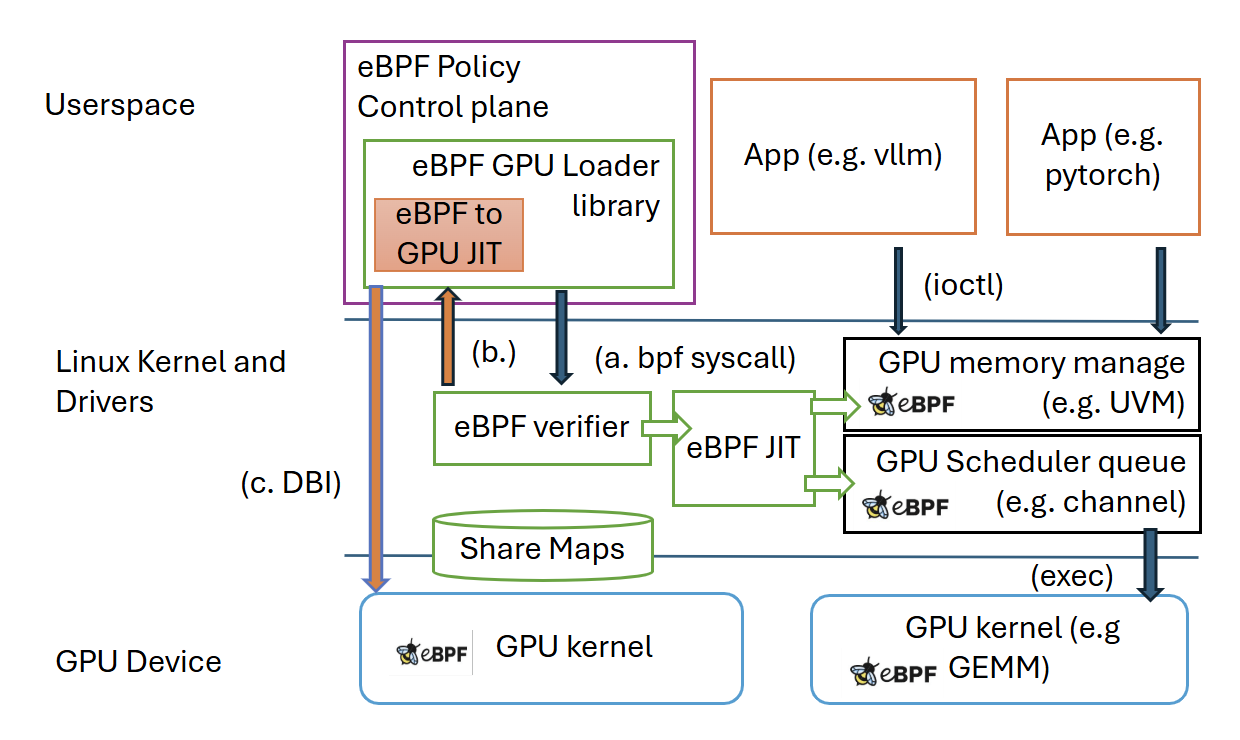
\includegraphics[width=\columnwidth]{img/gpu-ebpf-arch.png}
\vspace{-.5ex}
\caption{\sys architecture: cross-layer eBPF runtime spanning kernel driver and GPU device. The control plane deploys policies via (a) bpf syscall to verifier and driver hooks (b) GPU JIT after verification; (c) DBI injects trampolines into GPU kernels. Shared maps enable state coordination across layers.}
\label{fig:system-design}
\end{figure}

Figure~\ref{fig:system-design} shows the architecture of \sys.

% \sys exposes \emph{hierarchical cross-layer maps}: logical eBPF map abstractions whose backing storage is automatically partitioned and replicated across host DRAM, GPU global memory, and optionally per-SM scratch space, with consistency and placement managed transparently by the runtime. Policy developers access maps via standard eBPF helpers regardless of execution context, without manual DMA transfers, memory placement, or address translation.

\paragraph{User-space Control Plane.}
Policy authors use standard eBPF tooling (e.g., \texttt{clang/libbpf}, \texttt{bpftool}) to build policy bytecode. The control-plane links against a loader library that installs policies and configures eBPF maps. It enables runtime policy redeployment and reconfiguration (e.g., eviction thresholds, sampling rates, priorities) without application or kernel restarts, and exports runtime metrics (e.g., region hotness, tenant latencies).

\paragraph{Host Driver and Device Runtime.}
\sys provides a unified runtime across host driver and GPU device contexts, managing verification, compilation, and map placement. It employs a SIMT-aware verifier (\S\ref{sec:verification}) that extends standard eBPF checks to verify warp-uniformity, SIMT control flow, and GPU synchronization constraints. Verified programs are JIT-compiled into native host code or GPU-compatible instructions (e.g., PTX). The runtime manages hierarchical logical eBPF map abstractions whose backing storage is automatically partitioned and replicated across host and device with consistency.
Policy execution occurs at structured hook points defined in GPU drivers and device. On the host, \sysdriver exposes \texttt{struct\_ops}-style hooks (e.g., region activate/eviction, GPU kernel scheduling). Host policies return concise policy decisions enforced via trusted kfuncs. On the GPU device, \sys injects trampolines at hook points and invokes device-side handlers at warp granularity. Device handlers update cross-layer maps with performance signals and make control decisions (e.g., prefetch, block-level scheduling) via trusted helpers that the runtime enforces.

\subsection{\sys{} Policy Interfaces}
\label{sec:design-interfaces}

\sys introduces three eBPF program types: two in the driver‑level ( \texttt{BPF\_PROG\_TYPE\_GPU\_MEM} for memory‑placement policy and \texttt{BPF\_PROG\_TYPE\_GPU\_SCHED} for scheduling decisions), and one in the device‑level ( \texttt{BPF\_PROG\_TYPE\_GPU\_DEV} for GPU kernel instrumentation).
These program types coexist with existing kernel eBPF program types and have different SIMT‑specific verification rules.

\subsubsection{Memory Interface}
\label{sec:design-mem}

\sys treats memory placement as a programmable cache. It exposes four events (\emph{activate}, \emph{access}, \emph{evict\_prepare}, and \emph{prefetch}) and allows host and device policies to cooperate. \sys regions correspond to GPU hardware-managed units, such as 2MB physical UVM chunks or VA blocks, and finer-grained 4KB pages. This granularity balances policy precision against metadata overhead. Using the regions abstraction, \sys hides vendor-specific and hardware complexities. The host driver exports these events through a \texttt{struct\_ops} table. Handlers encode decisions through an enum field in the context and may reorder but never remove regions in the kernel‑maintained eviction list. The kernel enforces safety and correctness, including fallback FIFO eviction under pressure. Policies maintain their own metadata in maps and express placement and prefetch decisions through these handlers.

Device policies can be triggered at given memory operations and receive a compact warp‑uniform context. Operations like prefetch can be performed on device and then trigger host-side prefetch handlers, enabling the host to combine driver information with device‑side predictive logic. The following interface illustrates the host and device memory policy hooks:

\begin{lstlisting}
// Host-side policy handlers for GPU memory management
struct gpu_mem_ops {
  // Region created or eligible for device placement
  int (*gpu_activate)(gdrv_mem_add_ctx_t *ctx);
  // Memory subsystem observes region use;
  // decide cache hit/eviction policies
  int (*gpu_access)(gdrv_mem_access_ctx_t *ctx);
  // Region about to leave device-resident working set
  int (*gpu_evict_prepare)(gdrv_mem_remove_ctx_t *ctx);
  // Safe points (e.g. faults) for prefetch
  int (*gpu_prefetch)(gdrv_mem_prefetch_ctx_t *ctx);
};

// Host-side kfuncs: reorder regions in eviction list
void bpf_gpu_move_head(gdrv_mem_list_t *list,
                               gmem_region_t *r);
void bpf_gpu_move_tail(gdrv_mem_list_t *list,
                               gmem_region_t *r);

// Device-side memory handler interface
struct gdev_mem_ops {
    // Warp observed memory access;
    void (*access)(gdev_mem_access_ctx_t *ctx);
    // GPU kernel fence point
    void (*fence)(gdev_mem_fence_ctx_t *ctx);
};

// Device-side helpers
// Request prefetch, triggers handler in host driver
 int gdev_mem_prefetch(gmem_region_t* r);
\end{lstlisting}

\subsubsection{Scheduling Interface}
\label{sec:design-sched}

\sys exposes scheduling policy control at two levels: hardware‑queue lifecycle (host‑side) and thread‑block scheduling (device‑side). The host participates in GPU queue admission and priority control through policies. Policies set queue priority, timeslice, and may reject or defer queue creation. Properties are written directly into firmware‑visible structures, ensuring enforcement beyond user‑space hints. Policies may also invoke the \texttt{gdrv\_sched\_preempt} kfunc to trigger cooperative preemption through the driver's native context‑switch mechanism.

Within the GPU, \sys provides a work‑stealing thread‑block scheduler. GPU kernels expose their logical work units; persistent worker blocks select and process units while device‑side eBPF handlers steer scheduling decisions via \texttt{gdev\_block\_ctx}. The verifier ensures that scheduling decisions respect GPU kernel invariants (e.g., selecting only local work units). \sys can inject this scheduler via binary rewriting or allow developers to integrate it.

\begin{lstlisting}
// Host-side policy handlers for GPU hardware
// queue scheduling
struct gpu_sched_ops {
  // Hardware queue creation; set prio/timeslice,
  // return 0 to accept or <0 to reject/defer
  int  (*task_init)(gsched_queue_ctx_t *ctx);
  // Hardware queue destruction; cleanup policy
  void (*task_destroy)(gsched_queue_ctx_t *ctx);
};

// Host-side kfuncs
void bpf_gpu_set_attr(gsched_queue_ctx_t *ctx, u64 us);
void bpf_gpu_reject_bind(gsched_queue_ctx_t *ctx);

// Device-side block scheduling handlers
struct gdev_sched_ops {
  // Worker block starts/exits new work unit
  void (*enter)(gdev_block_ctx_t *ctx);
  void (*exit)(gdev_block_ctx_t *ctx);

  // Device function starts/ends
  void (*probe)(gdev_block_ctx_t *ctx);
  void (*retprobe)(gdev_block_ctx_t *ctx);

  // Return whether to steal work (TB scheduler)
  bool (*should_try_steal)(gdev_block_ctx_t *ctx);
};
\end{lstlisting}

\subsection{Runtime Verification and Optimizations}
\label{sec:verification}

\sys policies execute directly within privileged GPU driver and kernel contexts, making safety guarantees critical. We adopt a standard eBPF threat model: we trust system administrators loading policies, but consider policy code potentially buggy or misconfigured. The trusted computing base (TCB) includes the kernel and \sys kernel module, GPU compiler backend, and GPU driver/firmware. Policy authors only interact with eBPF and do not write native device code. For host-side verification, we reuse the existing Linux kernel eBPF verifier unchanged, relying on standard type-checking, bounded-loop, and memory-safety constraints. \sys-specific kfuncs and hooks are declared via BPF Type Format (BTF) metadata.

\subsubsection{SIMT-aware Verification}

To solve the SIMT mismatch described in C2, \sys introduces a SIMT-aware static verification model enforcing warp-level uniformity constraints to ensure efficient and safe GPU-side policy execution.
The key insight is that we distinguish \emph{warp-uniform} values (identical across warp threads, e.g., region identifiers) from \emph{lane-varying} values (thread-local GPU state). Policies may compute freely using lane-varying values, but these must not influence control-flow decisions or directly produce side effects visible outside a warp. To guarantee warp-level coherence, \sys mandates that branch conditions, loop bounds, and map-update keys be warp-uniform or derived via warp-level aggregation. Additionally, \sys prohibits GPU-wide barriers, global synchronization primitives, and non-uniform atomic operations, and imposes resource budgets per policy hook to bound memory and thread resource usage. These constraints ensure safe policy integration that respects GPU hardware execution semantics.

\subsubsection{Warp-level Execution Optimizations}

Direct scalar execution of eBPF after SIMT verification on GPU threads still causes resource overhead (e.g. duplicate memory update to maps) due to the SIMT. To resolve this, \sys introduces a warp-level aggregated execution model, executing policy logic once per warp using a designated "warp leader" (typically lane 0). Each hook invocation conceptually follows a two-phase approach: each lane independently computes lane-local contributions (e.g., effective addresses, counters) without influencing control flow or directly updating shared state. These contributions are then aggregated at warp granularity. Subsequently, the warp leader executes the policy handler once using aggregated inputs and warp-uniform context. The resulting decision is broadcast back to all lanes. This design minimizes GPU overhead while preserving eBPF's scalar semantics. To further reduce runtime overhead, \sys employs compiler-level optimizations (specialization and inlining) tailored for warp-level execution.

\subsubsection{Hierarchical Cross-layer Maps for State Coordination}

GPU policy decisions require coherent sharing of policy state across asynchronous CPU and GPU contexts. To transparently bridge CPU-GPU memory hierarchies, \sys introduces cross-layer maps. Logically, each map is a single unified key-value store accessible from host-side driver hooks, GPU-side device policies, and user-space control planes, and verifiable through eBPF's existing model. Physically, maps are realized as hierarchical shards across host DRAM, GPU global memory, and GPU-local storage (e.g., shared memory, SM-local). The runtime dynamically determines shard placement based on access frequency, latency, and capacity constraints. Following eBPF's soft-state philosophy, \sys maps provide relaxed, eventual consistency. Instead of strong global ordering, our runtime periodically merges GPU-local map shards into canonical snapshots at synchronization points, such as GPU kernel completion boundaries. This snapshot-based model is sufficient for policy decisions relying on approximate statistics. Occasional staleness affects decision optimality but cannot violate correctness invariants such as memory integrity, which remain enforced by the GPU driver and hardware MMU.
